\documentclass[aspectratio=169, table]{beamer}

\usepackage[utf8]{inputenc}
\usepackage{listings} 

\usetheme{Pradita}

\subtitle{Kuliah Umum}

\title{\LARGE{Lokakarya GIT}\\\vspace{10pt}}
\date[Serial]{\\\vspace{10pt}\scriptsize {Jumat, 27 September 2024}}
\author[Pradita]{\\\vspace{20pt}\small{\textbf{Alfa Yohannis}}}

% Define Java language style for listings
\lstdefinestyle{java}{
	language=Java,
	basicstyle=\ttfamily\footnotesize,
	keywordstyle=\color{blue},
	commentstyle=\color{gray},
	stringstyle=\color{red},
	breaklines=true,
	showstringspaces=false,
	tabsize=2,
	captionpos=b,
	numbers=left,
	numberstyle=\tiny\color{gray},
	comment=[l]{//},
	morecomment=[s]{/*}{*/},
	commentstyle=\color{gray}\ttfamily,
	string=[s]{'}{'},
	morestring=[s]{"}{"},
	%	stringstyle=\color{teal}\ttfamily,
	%	showstringspaces=false
}

\lstdefinelanguage{bash} {
	keywords={},
	basicstyle=\ttfamily\small,
	keywordstyle=\color{blue}\bfseries,
	ndkeywords={},
	ndkeywordstyle=\color{purple}\bfseries,
	sensitive=true,
	commentstyle=\color{gray},
	stringstyle=\color{red},
	numbers=left,
	numberstyle=\tiny\color{gray},
	breaklines=true,
	frame=lines,
	backgroundcolor=\color{lightgray!10},
	tabsize=2,
	comment=[l]{\#},
	morecomment=[s]{/*}{*/},
	commentstyle=\color{gray}\ttfamily,
	stringstyle=\color{purple}\ttfamily,
	showstringspaces=false
}


\begin{document}
	
	\frame{\titlepage}
	
	% Add table of contents slide
	\begin{frame}[fragile]{Contents (1)}
		\vspace{15pt}
		\begin{columns}[t]
			\begin{column}{.5\textwidth}
				\tableofcontents[sections={1-6}]
			\end{column}
			\begin{column}{.5\textwidth}
				\tableofcontents[sections={7-15}]
			\end{column}
		\end{columns}
	\end{frame}
	
	\begin{frame}[fragile]{Contents (2)}
		\vspace{15pt}
		\begin{columns}[t]
			\begin{column}{.5\textwidth}
				\tableofcontents[sections={16-24}]
			\end{column}
			\begin{column}{.5\textwidth}
				\tableofcontents[sections={25-50}]
			\end{column}
		\end{columns}
	\end{frame}
	
	\section{Pendahuluan}
	

\begin{frame}[fragile]
	\frametitle{Original Version}
	\begin{lstlisting}[style=java,basicstyle=\ttfamily]
public static void main(String[] args) {
	
	System.out.println("Hello World!");
	
}
	\end{lstlisting}
\end{frame}

	
\begin{frame}[fragile]
\frametitle{Many Versions}
\begin{columns}[t]
\begin{column}{.5\textwidth}
\textbf{My Version}
\begin{lstlisting}[style=java,basicstyle=\ttfamily\scriptsize]
public static void main(String[] args) {
	
	System.out.println("Hello, " 
		+ args[0]);
	
}
\end{lstlisting}
\end{column}
\begin{column}{.5\textwidth}
\textbf{Alice's Version}
\begin{lstlisting}[style=java,basicstyle=\ttfamily\scriptsize]
public static void main(String[] args) {
	if (args.length > 0) {
		System.out.println("Hello, " + args[0]);
	} else {
		System.out.println("Hello World!");
	}
}
\end{lstlisting}
\end{column}
\end{columns}

\end{frame}

	\begin{frame}[fragile]
	\frametitle{Branch Workflow}
	\vspace{25pt}
	\begin{center}
		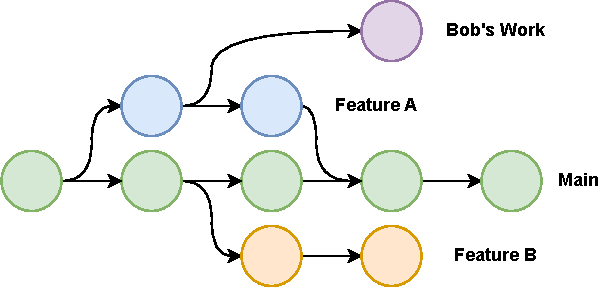
\includegraphics[width=.90\textwidth]{../images/branch}
	\end{center}
\end{frame}
	
	\begin{frame}[fragile]
		\frametitle{Operasi-operasi Git}
		\vspace{25pt}
		\begin{center}
			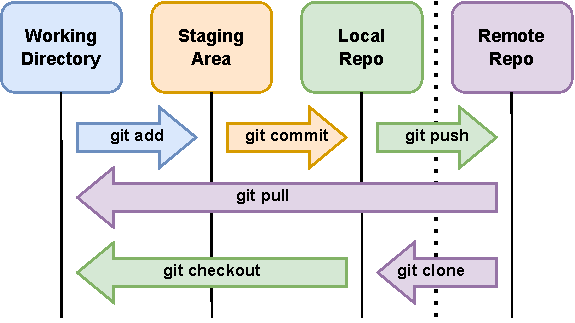
\includegraphics[width=.75\textwidth]{../images/diagram}
		\end{center}
	\end{frame}
	
	
	\begin{frame}[fragile]
		\frametitle{Apa itu Sistem Version Control?}
		\begin{itemize}
			\item Alat untuk mengelola perubahan pada kode sumber atau dokumen dari waktu ke waktu.
			\item Memungkinkan beberapa pengembang untuk berkolaborasi.
			\item Melacak perubahan dan mengembalikan ke versi sebelumnya jika diperlukan.
			\item Mencatat setiap perubahan yang dilakukan pada file.
			\item Memudahkan pelacakan evolusi proyek.
		\end{itemize}
	\end{frame}
	
	\begin{frame}[fragile]
		\frametitle{Manfaat Menggunakan VCS}
		\begin{itemize}
			\item \textbf{Kolaborasi}: 
			\begin{itemize}
				\item Beberapa anggota tim dapat bekerja secara bersamaan tanpa saling menimpa pekerjaan.
			\end{itemize}
			\item \textbf{Riwayat}: 
			\begin{itemize}
				\item Setiap perubahan dicatat, memberikan riwayat lengkap modifikasi.
			\end{itemize}
			\item \textbf{Kemampuan Mengembalikan}: 
			\begin{itemize}
				\item Mengembalikan ke versi sebelumnya jika terjadi kesalahan.
			\end{itemize}
			\item \textbf{Branching dan Merging}: 
			\begin{itemize}
				\item Fitur atau perbaikan dapat dikembangkan secara terpisah.
				\item Dapat digabungkan kembali ke proyek utama setelah selesai.
			\end{itemize}
		\end{itemize}
	\end{frame}
	
	\section{Jenis-jenis Sistem Version Control}
	
	\subsection{Local Version Control System (LVCS)}
	
	\begin{frame}[fragile]
		\frametitle{Local Version Control System (LVCS)}
		\begin{itemize}
			\item Menyimpan semua versi file secara lokal di komputer pengguna.
			\item Salinan file dibuat secara manual di direktori berbeda.
			\item Metode ini rentan terhadap kesalahan.
			\item \textbf{Contoh produk}:
			\begin{itemize}
				\item File system sederhana untuk membuat salinan file secara manual.
			\end{itemize}
		\end{itemize}
	\end{frame}
	
	\subsection{Centralized Version Control System (CVCS)}
	
	\begin{frame}[fragile]
		\frametitle{Centralized Version Control System (CVCS)}
		\begin{itemize}
			\item Menggunakan server pusat untuk menyimpan semua versi file.
			\item Pengguna harus terhubung ke server untuk mendapatkan atau memperbarui versi file.
			\item Mempermudah kolaborasi.
			\item Kelemahan: risiko kegagalan server pusat.
			\item \textbf{Contoh produk}:
			\begin{itemize}
				\item \textbf{Subversion (SVN)}: Sistem version control terpusat yang populer.
				\item \textbf{Perforce}: Sistem VCS yang digunakan oleh perusahaan besar.
				\item \textbf{CVS (Concurrent Versions System)}: Sistem version control yang lebih tua.
			\end{itemize}
		\end{itemize}
	\end{frame}
	
	\subsection{Distributed Version Control System (DVCS)}
	
	\begin{frame}[fragile]
		\frametitle{Distributed Version Control System (DVCS)}
		\begin{itemize}
			\item Setiap pengguna memiliki salinan lengkap dari seluruh riwayat proyek.
			\item Pengguna dapat bekerja secara offline.
			\item Perubahan dapat digabungkan dengan server pusat atau pengguna lain.
			\item \textbf{Contoh produk}:
			\begin{itemize}
				\item \textbf{Git}: Sistem version control terdistribusi yang paling populer.
				\item \textbf{Mercurial}: Alternatif untuk Git.
				\item \textbf{Bazaar}: Sistem VCS yang digunakan di beberapa komunitas open-source.
			\end{itemize}
		\end{itemize}
	\end{frame}
	
	\section{Latar Belakang Git}
	
	\begin{frame}[fragile]
		\vspace{10pt}
		\frametitle{Latar Belakang Git}
		Git adalah sistem version control terdistribusi, yang awalnya dikembangkan oleh Linus Torvalds pada tahun 2005 untuk mengelola pengembangan kernel Linux. 
		
		\textbf{Tujuan desain utama Git}:
		\begin{itemize}
			\item \textbf{Kecepatan}: Penanganan tugas-tugas version control dengan cepat.
			\item \textbf{Desain Sederhana}: Git dirancang agar mudah digunakan namun kuat.
			\item \textbf{Dukungan Kuat untuk Pengembangan Non-linear}: Kemampuan branching dan merging yang kuat.
			\item \textbf{Pengembangan Terdistribusi}: Setiap pengembang memiliki salinan penuh dari sejarah proyek secara lokal.
		\end{itemize}
	\end{frame}
	
	\section{Instal Git Secara Lokal}
	
	
	\subsection{Menginstal Git di Linux}
	
	\begin{frame}[fragile]
		\frametitle{Menginstal Git di Linux}
		\begin{itemize}
			\item Untuk Debian/Ubuntu:
			\begin{lstlisting}[language=bash]
				sudo apt-get install git
			\end{lstlisting}
			\item Untuk Red Hat:
			\begin{lstlisting}[language=bash]
				sudo yum install git
			\end{lstlisting}
			\item Verifikasi instalasi:
			\begin{lstlisting}[language=bash]
				git --version
			\end{lstlisting}
		\end{itemize}
	\end{frame}
	
	\section{Membuat Akun GitHub}
	
	\begin{frame}[fragile]
		\frametitle{Membuat Akun GitHub}
		GitHub adalah platform populer untuk menghosting repository Git di cloud.
		\begin{enumerate}
			\item Buka \url{https://github.com/} dan klik tombol \texttt{Sign up}.
			\item Isi detail yang diperlukan.
			\item Verifikasi email dan selesaikan proses pembuatan akun.
			\item Setelah masuk, mulai membuat repository dan berkolaborasi.
		\end{enumerate}
	\end{frame}
	
	\section{Git Init: Menginisialisasi Repository}
	
	\begin{frame}[fragile]
		\frametitle{Git Init: Menginisialisasi Repository}
		\vspace{15pt}
		\begin{itemize}
			\item Perintah \texttt{git init} digunakan untuk menginisialisasi repository Git baru.
			\item Membuat direktori \texttt{.git} di dalam folder proyek.
			\item Direktori \texttt{.git} menyimpan semua metadata dan riwayat version control.
			\item Perintah:
			\begin{lstlisting}[language=bash]
				git init
			\end{lstlisting}
			\item Setelah dijalankan, folder proyek menjadi repository Git dan siap untuk melacak perubahan.
		\end{itemize}
	\end{frame}
	
	\section{Git Add: Menambahkan Perubahan ke Staging}
	
	\begin{frame}[fragile]
		\frametitle{Git Add: Menambahkan Perubahan ke Staging}
		\vspace{15pt}
		\begin{itemize}
			\item Perintah \texttt{git add} digunakan untuk menambahkan perubahan pada file ke area staging.
			\item Area staging adalah tahap sebelum perubahan dikomit ke repository.
			\item File individu atau semua file yang diubah bisa ditambahkan sekaligus.
			\item Perintah:
			\begin{lstlisting}[language=bash]
				git add <nama_file>
				git add .
			\end{lstlisting}
			\item Menggunakan \texttt{git add .} menambahkan semua file yang berubah ke staging.
		\end{itemize}
	\end{frame}
	
	\section{Git Commit: Mengkomit Perubahan}
	
	\begin{frame}[fragile]
		\frametitle{Git Commit: Mengkomit Perubahan}
		\begin{itemize}
			\item Perintah \texttt{git commit} digunakan untuk mengunci perubahan ke dalam repository.
			\item Setiap \texttt{commit} memerlukan pesan yang menjelaskan perubahan.
			\item Perintah:
			\begin{lstlisting}[language=bash]
				git commit -m "Deskripsi perubahan"
			\end{lstlisting}
			\item Pesan commit harus jelas untuk memudahkan pelacakan riwayat perubahan.
		\end{itemize}
	\end{frame}
	
	\section{Git Reset: Menghapus Perubahan dari Staging}
	\begin{frame}[fragile]
		\frametitle{Git Reset: Menghapus Perubahan dari Staging}
		\begin{itemize}
			\item Gunakan perintah \texttt{git reset} untuk membatalkan perubahan yang telah ditambahkan ke staging.
			\item Tanpa mengubah file yang sebenarnya.
			\item Perintah:
			\begin{lstlisting}[language=bash]
				git reset <nama_file>
			\end{lstlisting}
			\item Menghapus file dari staging, tetapi perubahan tetap ada.
			\item Untuk membatalkan perubahan pada file, gunakan \texttt{git checkout}.
		\end{itemize}
	\end{frame}
	
	\section{Penggunaan File .gitignore}
	
	\begin{frame}[fragile]
		\frametitle{Penggunaan File .gitignore}
		\begin{itemize}
			\item File \texttt{.gitignore} menentukan file atau direktori yang tidak ingin dilacak.
			\item Pola atau nama file yang tidak akan ditambahkan ke staging meskipun diubah.
			\item Contoh file \texttt{.gitignore}:
			\begin{lstlisting}[language=bash]
				# Contoh file .gitignore
				node_modules/
				*.log
				*.tmp
			\end{lstlisting}
			\item Dengan menambahkan pola, Git akan mengabaikan file-file tersebut.
		\end{itemize}
	\end{frame}
	
	\section{Membuat dan Menggabungkan Branch}
	
	\begin{frame}[fragile]
		\frametitle{Membuat Branch}
		\begin{itemize}
			\item Git memungkinkan pekerjaan pada berbagai fitur atau perbaikan menggunakan \textit{branch}.
			\item Perintah \texttt{git branch} untuk membuat cabang baru.
			\item Perintah \texttt{git checkout} untuk berpindah ke cabang tersebut.
			\item Perintah:
			\begin{lstlisting}[language=bash]
				git branch <nama_branch>
				git checkout <nama_branch>
			\end{lstlisting}
		\end{itemize}
	\end{frame}
	
	\begin{frame}[fragile]
		\frametitle{Menggabungkan Branch}
		\begin{itemize}
			\item Setelah perubahan selesai, cabang bisa digabungkan ke cabang utama.
			\item Perintah untuk menggabungkan:
			\begin{lstlisting}[language=bash]
				git checkout main
				git merge <nama_branch>
			\end{lstlisting}
			\item Menggabungkan perubahan dari cabang lain ke dalam cabang utama.
		\end{itemize}
	\end{frame}
	
	\section{Membuat Repository Private/Public}
	
	\begin{frame}[fragile]
		\frametitle{Membuat Repository di GitHub}
		\begin{itemize}
			\item GitHub memungkinkan pembuatan repository private dan public untuk mengelola proyek.
			\item Langkah-langkah untuk membuat repository:
			\begin{enumerate}
				\item Masuk ke akun GitHub dan klik tombol \texttt{New Repository}.
				\item Berikan nama repository dan deskripsi opsional.
				\item Pilih sifat repository:
				\begin{itemize}
					\item \texttt{Public}: dapat diakses oleh siapa saja.
					\item \texttt{Private}: hanya bisa diakses oleh pemilik dan kolaborator yang diizinkan.
				\end{itemize}
				\item Pilih opsi tambahan: \texttt{README.md}, \texttt{.gitignore}, atau lisensi.
				\item Klik \texttt{Create repository}.
			\end{enumerate}
		\end{itemize}
	\end{frame}
	
	\section{Menambahkan Remote dan Push Perubahan}
	
	\begin{frame}[fragile]
		\frametitle{Menambahkan Remote}
		\begin{itemize}
			\item Setelah membuat repository di GitHub, langkah selanjutnya adalah menambahkan repository tersebut sebagai \textit{remote} di proyek Git lokal.
			\item Untuk menambahkan remote:
			\begin{itemize}
				\item Gunakan perintah:
				\begin{lstlisting}[language=bash]
					git remote add origin https://github.com/username/nama-repo.git
				\end{lstlisting}
				\item \texttt{origin} adalah nama default untuk remote repository utama.
				\item Nama lain dapat digunakan jika diinginkan.
			\end{itemize}
		\end{itemize}
	\end{frame}
	
	\begin{frame}[fragile]
		\frametitle{Push Perubahan ke Remote}
		\begin{itemize}
			\item Setelah remote ditambahkan, kirim perubahan dari repository lokal ke GitHub.
			\item Gunakan perintah:
			\begin{lstlisting}[language=bash]
				git push -u origin main
			\end{lstlisting}
			\item Perintah ini mengirim semua commit di cabang \texttt{main} ke remote \texttt{origin}.
			\item Opsi \texttt{-u} mengatur \texttt{main} sebagai cabang default untuk operasi \texttt{push} berikutnya.
		\end{itemize}
	\end{frame}
	
	\begin{frame}[fragile]
		\frametitle{Sinkronisasi Perubahan}
		\begin{itemize}
			\item Untuk menarik (pull) perubahan dari repository remote ke lokal, gunakan perintah:
			\begin{lstlisting}[language=bash]
				git pull origin main
			\end{lstlisting}
			\item Perintah ini memastikan repository lokal tetap sinkron dengan repository GitHub.
		\end{itemize}
	\end{frame}
	
	\section{Memfork Repository}
	
	\begin{frame}[fragile]
		\frametitle{Memfork Repository}
		\begin{itemize}
			\item Memfork repository memungkinkan pengguna membuat salinan pribadi dari proyek orang lain.
			\item Memungkinkan eksperimen dan modifikasi tanpa mempengaruhi proyek asli.
			\item Langkah-langkah untuk memfork repository:
			\begin{enumerate}
				\item Arahkan ke repository GitHub yang ingin difork.
				\item Klik tombol \texttt{Fork} di bagian kanan atas halaman.
				\item Pilih akun sebagai tujuan untuk repository yang difork.
			\end{enumerate}
			\item Setelah memfork, salinan baru dibuat di bawah akun GitHub.
		\end{itemize}
	\end{frame}
	
	\section{Mengkloning Repository}
	
	\begin{frame}[fragile]
		\frametitle{Mengkloning Repository}
		\begin{itemize}
			\item Mengkloning repository memungkinkan pengguna mengunduh salinan repository ke mesin lokal.
			\item Gunakan perintah berikut di terminal:
			\begin{lstlisting}[language=bash]
				git clone <repository-url>
			\end{lstlisting}
			\item Gantilah \texttt{<repository-url>} dengan URL dari repository yang difork atau asli.
			\item Perintah ini membuat salinan lokal untuk bekerja secara offline.
		\end{itemize}
	\end{frame}
	
	\section{Membuat Pull Request}
	
	\begin{frame}[fragile]
		\frametitle{Membuat Pull Request}
		\vspace{20pt}
		\begin{itemize}
			\item Setelah melakukan perubahan pada repository yang dikloning, langkah berikutnya adalah mengirimkan perubahan untuk ditinjau.
			\item Langkah-langkah untuk membuat pull request:
			\begin{enumerate}
				\item Dorong perubahan ke repository yang difork:
				\begin{lstlisting}[language=bash]
					git push origin <branch-name>
				\end{lstlisting}
				\item Buka repository asli di GitHub.
				\item Klik pada tab \texttt{Pull requests}.
				\item Klik tombol \texttt{New pull request}.
				\item Pilih cabang dan berikan deskripsi tentang perubahan.
				\item Klik \texttt{Create pull request}.
			\end{enumerate}
			\item Pull request memfasilitasi diskusi dan tinjauan sebelum digabungkan.
		\end{itemize}
	\end{frame}
	
	\section{Mengambil dan Mengirim Perubahan di GitHub}
	
	\begin{frame}[fragile]
		\frametitle{Mengambil dan Mengirim Perubahan}
		\begin{itemize}
			\item Untuk menyinkronkan perubahan antara repository lokal dan jarak jauh:
			\begin{itemize}
				\item Mengambil perubahan terbaru dari repository jarak jauh:
				\begin{lstlisting}[language=bash]
					git pull origin <branch-name>
				\end{lstlisting}
				\item Mengirim perubahan lokal ke repository jarak jauh:
				\begin{lstlisting}[language=bash]
					git push origin <branch-name>
				\end{lstlisting}
			\end{itemize}
			\item Perintah ini memastikan semua kontributor bekerja dengan versi kode terbaru.
		\end{itemize}
	\end{frame}
	
	\section{Menyelesaikan Konflik Penggabungan}
	
	\begin{frame}[fragile]
		\frametitle{Menyelesaikan Konflik Penggabungan (1)}
		\vspace{20pt}
		\begin{itemize}
			\item Konflik penggabungan dapat terjadi jika beberapa kontributor melakukan perubahan pada bagian yang sama.
			\item Langkah-langkah untuk menyelesaikan konflik:
			\begin{enumerate}
				\item Ambil perubahan terbaru dari repository jarak jauh.
				\item Jika terjadi konflik, Git akan menandai file yang konflik.
				\item Buka file yang konflik dan cari penanda konflik (misalnya, \texttt{<<<<<<< HEAD}).
				\item Edit file secara manual untuk menyelesaikan konflik.
			\end{enumerate}
		\end{itemize}
	\end{frame}
	
	\begin{frame}[fragile]
		\frametitle{Menyelesaikan Konflik Penggabungan (2)}
		\vspace{20pt}
		\begin{itemize}
			\item Setelah menyelesaikan konflik, siapkan perubahan:
			\begin{lstlisting}[language=bash]
				git add <resolved-file>
			\end{lstlisting}
			\item Komit perubahan yang telah diselesaikan:
			\begin{lstlisting}[language=bash]
				git commit -m "Resolved merge conflict"
			\end{lstlisting}
			\item Langkah-langkah ini membantu mengelola dan menyelesaikan konflik penggabungan.
		\end{itemize}
	\end{frame}
	
	
	\section{Hindari Mengunggah File Binary Target}
	\begin{frame}[fragile]
		\frametitle{Hindari Mengunggah File Binary Target}
		\begin{itemize}
			\item File binary target, seperti file hasil kompilasi atau executable, sebaiknya tidak diunggah ke repository.
			\item File tersebut dapat cepat membesar dan tidak perlu dilacak di dalam version control.
			\item Simpan kode sumbernya dan biarkan setiap pengguna melakukan kompilasi di mesin masing-masing.
		\end{itemize}
	\end{frame}
	
	\section{Hindari File Binary Berukuran Besar}
	\begin{frame}[fragile]
		\frametitle{Hindari File Binary Berukuran Besar}
		\begin{itemize}
			\item File binary besar, seperti gambar, video, atau file media lainnya, sebaiknya dihindari.
			\item Gunakan platform penyimpanan eksternal seperti Git LFS atau layanan penyimpanan awan.
			\item Ini membantu menjaga ukuran repository tetap kecil dan mudah dikelola.
		\end{itemize}
	\end{frame}
	
	\section{Hindari File Temporary}
	\begin{frame}[fragile]
		\frametitle{Hindari File Temporary}
		\begin{itemize}
			\item File sementara yang dihasilkan selama pengembangan, seperti file log, cache, atau konfigurasi lokal, sebaiknya tidak diunggah.
			\item Gunakan file \texttt{.gitignore} untuk mengabaikan file-file ini agar tidak termasuk dalam version control.
		\end{itemize}
		\begin{lstlisting}[language=bash]
			# Contoh isi .gitignore
			*.log
			*.tmp
			*.cache
		\end{lstlisting}
	\end{frame}
	
	\section{Tulis Pesan \textit{Commit} yang Jelas}
	\begin{frame}[fragile]
		\frametitle{Tulis Pesan \textit{Commit} yang Jelas}
		\begin{itemize}
			\item Pesan commit yang jelas dan deskriptif memudahkan pengembang lain memahami perubahan.
			\item Gunakan kalimat yang menjelaskan apa yang diubah dan mengapa.
		\end{itemize}
		\begin{lstlisting}[language=bash]
			git commit -m "Memperbaiki bug pada fungsi login dan menambahkan validasi input"
		\end{lstlisting}
	\end{frame}
	
	\section{Gunakan Branch untuk Fitur Baru dan Perbaikan}
	\begin{frame}[fragile]
		\frametitle{\LARGE{Gunakan Branch untuk Fitur Baru dan Perbaikan}}
		\begin{itemize}
			\item Selalu buat branch baru untuk mengembangkan fitur baru atau melakukan perbaikan.
			\item Ini menjaga cabang utama tetap stabil dan menghindari konflik yang tidak perlu.
		\end{itemize}
		\begin{lstlisting}[language=bash]
			git checkout -b nama_fitur_baru
		\end{lstlisting}
	\end{frame}
	
	\section{Jaga \textit{Commit} yang Kecil dan Sering}
	\begin{frame}[fragile]
		\frametitle{Jaga \textit{Commit} yang Kecil dan Sering}
		\begin{itemize}
			\item Commit yang kecil dan sering lebih mudah dikelola dan ditelusuri.
			\item Memudahkan pengembalian perubahan jika terjadi kesalahan.
		\end{itemize}
	\end{frame}
	
	\section{Perbarui \texttt{README.md} Secara Berkala}
	\begin{frame}[fragile]
		\frametitle{Perbarui \texttt{README.md} Secara Berkala}
		\begin{itemize}
			\item File \texttt{README.md} adalah dokumen penting yang menjelaskan proyek.
			\item Pastikan informasi di dalamnya selalu diperbarui, termasuk petunjuk instalasi, penggunaan, dan dokumentasi lainnya.
		\end{itemize}
	\end{frame}
	
	\section{Gunakan Pull Request untuk Kolaborasi}
	\begin{frame}[fragile]
		\frametitle{Gunakan Pull Request untuk Kolaborasi}
		\begin{itemize}
			\item Gunakan fitur pull request untuk mengusulkan perubahan saat bekerja dalam tim.
			\item Memfasilitasi diskusi dan tinjauan sebelum perubahan diterapkan ke cabang utama.
		\end{itemize}
	\end{frame}
	
	\section{Bersihkan Repository Secara Berkala}
	\begin{frame}[fragile]
		\frametitle{Bersihkan Repository Secara Berkala}
		\begin{itemize}
			\item Lakukan pemeriksaan rutin pada repository untuk menghapus file yang tidak diperlukan.
			\item Termasuk menghapus branch yang sudah tidak digunakan dan memperbarui file \texttt{.gitignore}.
		\end{itemize}
	\end{frame}
	
	\section{Patuhi Konvensi Penamaan}
	\begin{frame}[fragile]
		\frametitle{Patuhi Konvensi Penamaan}
		\begin{itemize}
			\item Gunakan konvensi penamaan yang konsisten untuk branch, commit, dan file.
			\item Memudahkan pengembang lain memahami struktur dan tujuan dari setiap elemen di dalam repository.
		\end{itemize}
	\end{frame}
	
	\begin{frame}
		\centering
		\Huge Q \& A
	\end{frame}
	
\end{document}
